% Author-guided revision, confined to manuscript/consolidation.
% Build: python ../work/readability_revision_20261114/03_build.py (from this directory).
\documentclass[journal]{IEEEtran}
\usepackage[T1]{fontenc}
\usepackage{amsmath,amssymb,amsthm,graphicx,booktabs,cite,array,multirow}
\usepackage{algorithm,algpseudocode,microtype,url}
\usepackage[hidelinks]{hyperref}
\hypersetup{pdftitle={Constructive and Destructive Training Regimes: From Gradient Interactions to Functional Oscillations},pdfauthor={Thiago Mattar; Cristiano L. Castro; Frederico Coelho; Yan G. Ferreira; Antonio P. Braga}}
\interdisplaylinepenalty=2500
\newtheorem{proposition}{Proposition}
\newcommand{\E}{\mathbb{E}}
\newcommand{\R}{\mathbb{R}}
\newcommand{\evidence}{../evidence}
\newcommand{\vcassetroot}{../evidence/05-adam/c-intervention}
\hyphenation{Wiki-Text Transformer pre-con-di-tion-er}
\title{Constructive and Destructive Training Regimes: From Gradient Interactions to Functional Oscillations}
\author{Thiago Mattar, Cristiano L. Castro, Frederico Coelho, Yan G. Ferreira, Antonio P. Braga%
\thanks{Thiago Mattar and Yan G. Ferreira are with the Graduate Program in Electrical Engineering, Universidade Federal de Minas Gerais, Belo Horizonte 31270-901, Brazil (e-mail: thiagocmattar@gmail.com; yanvgferreira@gmail.com).}%
\thanks{Cristiano L. Castro is with the Graduate Program in Electrical Engineering and the Department of Electrical Engineering, Universidade Federal de Minas Gerais (UFMG), Belo Horizonte, Minas Gerais 31270-901, Brazil (e-mail: crislcastro@gmail.com).}%
\thanks{Frederico Coelho and Antonio P. Braga are with the Graduate Program in Electrical Engineering and the Department of Electronic Engineering, Universidade Federal de Minas Gerais (UFMG), Belo Horizonte, Minas Gerais 35931-008, Brazil (e-mail: fredgfc@ufmg.br; apbraga@ufmg.br).}}
\markboth{Constructive and Destructive Training Regimes}{Mattar et al.: Constructive and Destructive Training Regimes}
\begin{document}
\maketitle
\begin{abstract}
Neural networks can continue learning while successive gradients nearly reverse direction. Understanding when this oscillation remains productive requires connecting local optimization geometry to accumulated parameter change and to movement of the learned function. We characterize constructive and destructive training regimes through gradient alignment and magnitude, distinguishing local reversal from cumulative displacement and loss reduction. Under smooth full-batch gradient descent, a scalar computed from two existing gradients equals the step-averaged directional Hessian curvature; we give its pointwise approximation error and explicit sampling-noise contribution. Controlled experiments with multilayer perceptrons, residual networks, and Transformers show that negative adjacent interaction can coexist with positive total cross-step interaction and lower training loss. We then interpret the same observable under Adam as a projected gradient response and evaluate its association with future loss increases, retaining missed events and false alarms. A fixed-probe tracing algorithm reveals concentrated representation motion, shared temporal structure across depth, and repeated reversals along leading output patterns. Finally, a common-state comparison of learning-rate reduction, second-moment changes, gradient clipping, and local affine-displacement caps tests the functional interpretation. Across three single-initialization cases, the preselected median cap reduces mean training loss by 32.2\%, 9.4\%, and 19.8\%, while reversals persist. Endpoint and held-out tradeoffs limit the conclusion to controlled training dynamics. The resulting framework connects interaction, curvature, and functional movement without equating oscillation with failed learning.
\end{abstract}

\begin{IEEEkeywords}
Training dynamics, gradient alignment, directional curvature, representation learning, adaptive optimization.
\end{IEEEkeywords}
\raggedbottom
\section{Introduction}
\label{sec:introduction}

Neural scaling laws have ushered in new paradigms for interpreting deep learning dynamics. These laws relate performance gains to model size, dataset scale, and compute, motivating longer training horizons under tight efficiency constraints~\cite{hestness2017deep,kaplan2020scaling,henighan2020scaling,hoffmann2022chinchilla}. In this regime, optimization stability becomes an important practical requirement, since unstable training may result in slow convergence and high sensitivity to hyperparameter choices. In practice, stability is often maintained through a set of heuristics, such as momentum, batch-size scaling, normalization, weight decay, and learning-rate schedules~\cite{goyal2017accurate,smith2017cyclical,loshchilov2016sgdr,ioffe2015batch,krogh1991simple}. Despite their effectiveness, understanding when these mechanisms help, and when they fail, remains consequential for the design of training procedures.

Training can become unstable when updates are too large relative to sharp directions of the loss landscape, so that they overshoot rather than converge toward a minimum~\cite{polyak1964methods,bertsekas1997nonlinear}. Stochastic extensions, such as the break-even point framework, relate instability to both sharpness and curvature variability, particularly during an early phase in which learning rate and batch size shape the subsequent trajectory~\cite{jastrzebski2020break}. The Edge-of-Stability literature, however, shows that deep networks often continue to make progress near, or even beyond, the nominal sharpness threshold~\cite{cohen2021edge,arora2022understanding,damian2023self}. These works provide an important geometric interpretation of training dynamics. They also motivate a complementary question: how does one update interact with the next, and how do their repeated interactions affect learning? A trajectory can repeatedly reverse in some directions while continuing to descend in others. Explaining this behavior requires following both the magnitude and direction of the steps actually taken, rather than treating every oscillation as failed progress.

To examine these interactions, we characterize constructive and destructive training regimes through consecutive-gradient alignment and gradient magnitude. Persistent positive alignment, $\rho_t>0$, identifies a constructive regime in which successive SGD steps reinforce one another, whereas persistent negative alignment, $\rho_t<0$, identifies a destructive regime in which successive steps partially reverse preceding parameter changes. We connect these regimes to directional curvature and introduce an inexpensive estimate of curvature along the step taken. It uses consecutive gradients and the actual parameter change, so the formulation applies to SGD, Adam, and other optimizers without additional Hessian computations. Under plain SGD, it reduces to a combination of gradient norms and their inner product. The formulation also makes the contribution of mini-batch sampling explicit, clarifying how noise affects the observed alignment and curvature estimate.

Destructive alignment alone does not imply instability. Within a local quadratic approximation, reversal and gradient growth jointly determine whether an SGD step decreases or increases the loss. This relationship explains how destructive regimes can sustain oscillatory descent, while sufficiently amplified reversals can produce upward loss excursions. Reading alignment and gradient norms together therefore provides a geometric interpretation of signals already available during training. Normalized displacement complements this local view by measuring how much of the total distance traveled remains as net parameter change.

We examine these relationships through controlled full-batch and mini-batch experiments across image-classification and language-modeling tasks, using multilayer perceptrons, residual networks, and Transformers. The SGD experiments isolate curvature and sampling effects. The Adam experiments then follow the argument from consecutive-gradient behavior to loss spikes, from spikes to changes in the network's representations, and from those changes to interventions. Evaluating the same reference examples at successive training steps makes it possible to see where representations reverse and where their changes become large. This motivates a local displacement cap, which we compare with learning-rate reduction, second-moment changes, and global gradient clipping from the same training states.

Our central contribution is to connect the interaction between training
steps to its consequences in parameter space, in the loss, and in the
learned function. This connection provides both an interpretation of
oscillatory progress and a measurable basis for intervention. Specifically:
\begin{itemize}
\item \textbf{Relating local reversal to accumulated learning dynamics.}
Edge-of-Stability studies establish that oscillation can coexist with
progress~\cite{cohen2021edge,damian2023self}, while gradient-product
diagnostics identify transitions toward
stationarity~\cite{chee2018diagnostics,pesme2020diagnostics}. These findings
motivate distinguishing opposition between neighboring updates from
cancellation across the complete trajectory. We connect consecutive-gradient
alignment to an exact all-pair displacement decomposition and normalized
displacement. The GD experiments show that negative adjacent interactions
can coexist with positive total interaction and decreasing loss, explaining
why a destructive local regime need not imply failed progress
(Sections~\ref{sec:displacement}--\ref{sec:gd-experiments}).

\item \textbf{Measuring curvature along the step actually taken.}
The leading Hessian eigenvalue used in spectral stability
analysis~\cite{cohen2021edge} describes the sharpest direction, but does not
specify the curvature encountered by a particular optimizer update.
We introduce an inexpensive step-direction estimate from consecutive
gradients and the applied parameter change, without additional backward
passes or Hessian computations. For smooth full objectives, we establish
its exact step-average interpretation independently of the optimizer,
including Adam, and bound its starting-point approximation error. Its
SGD specialization exposes the roles of alignment, norm growth, and
sampling noise; independently computed Hessian--vector products test
that interpretation (Sections~\ref{subsec:curvature-diagnostic}
and~\ref{subsec:gd-validation}).

\item \textbf{Separating gradient reversal from loss-spike formation.}
Bai et al.~\cite{bai2026spikes} explain Adam spikes through adaptive
preconditioning and gradient-directional curvature. To connect spike
behavior to consecutive training gradients, we express the local SGD
loss-increase condition jointly in terms of reversal and norm growth,
then examine those quantities under Adam without transferring the SGD
threshold into an Adam guarantee. An exhaustive comparison across
loss-increase magnitudes and future steps identifies both the association
and its missed increases and false alarms, extending the characterization
beyond selected peaks (Sections~\ref{subsec:loss}
and~\ref{subsec:characterization}).

\item \textbf{Tracing functional oscillation and testing selective control.}
Representation-change correction~\cite{kosson2024warmup} and unit-wise
gradient clipping~\cite{brock2021normalization} already motivate controlling
update size. We examine where successive representation changes reverse,
which patterns carry their movement, and whether limiting that movement
improves an oscillatory trajectory. Tracing the same reference examples
reveals concentrated movement and shared temporal structure across
measured stages. We then cap the direct affine displacement induced by
Adam's proposal using an absolute per-unit budget. Matched comparisons
with learning-rate reduction, second-moment changes, and global clipping
show lower mean training loss and positive loss variation for all tested
cap quantiles in the three cases, while reversals persist. Endpoint,
held-out, and cost tradeoffs delimit this training-dynamics result
(Sections~\ref{subsec:tracing}--\ref{sec:vc-interventions}).
\end{itemize}

The remainder of the paper is organized as follows. Section~\ref{sec:background} reviews training-stability perspectives. Section~\ref{sec:displacement} develops the displacement formulation and its diagnostics. Section~\ref{sec:gd-experiments} examines full-batch GD and mini-batch sampling. Section~\ref{sec:adam} develops the Adam characterization, representation analysis, and interventions. Section~\ref{sec:conclusion} concludes.

\section{Stability Analysis of SGD}
\label{sec:background}

Intuitively, smooth optimization occurs when updates reinforce each other
and gradually shift parameters toward a minimum of the loss. Larger steps
can overshoot, oscillate, and partially undo preceding parameter changes.
Understanding when such behavior remains productive, and when it produces
instability, requires examining how successive updates interact. Two factors
are central to this analysis: the \textit{local curvature} of the loss
landscape and the \textit{stochasticity} introduced by mini-batch sampling.

\subsection{Local Curvature of the Loss Function and Stability}

Training is a discrete-time dynamical system whose local response depends
on curvature. A step that produces smooth descent in a shallow direction
can overshoot in a sharper one. The Hessian quantifies this directional variation. Classical
analyses~\cite{polyak1964methods, bertsekas1997nonlinear} connect its
eigenvalues to the learning rate and local stability.

Let $\theta_t\in\mathbb{R}^p$ denote the parameters after $t$ completed updates and
$g_t$ a mini-batch gradient evaluated at $\theta_t$. Thus $g_t$ is available before
the next update, from $t$ to $t+1$. For a constant
learning rate $\eta>0$, plain SGD follows
\begin{equation}
  \theta_{t+1}=\theta_t-\eta g_t.
  \label{eq:sgd_map_stability}
\end{equation}
For full-batch GD, $g_t=\nabla\mathcal L(\theta_t)$. With
$H_t:=\nabla^2\mathcal L(\theta_t)$, the Jacobian of its update map is
\begin{equation}
  J_t=I-\eta H_t.
  \label{eq:jacobian_sgd}
\end{equation}
On a fixed quadratic objective, a perturbation along a Hessian eigendirection
is multiplied by $1-\eta\lambda_i$ at each step. For a positive-definite
Hessian, all components contract precisely when
\begin{equation}
  \max_i|1-\eta\lambda_i|<1
  \quad\Longleftrightarrow\quad
  \eta\lambda_{\max}(H_t)<2.
  \label{eq:quad_stability_condition}
\end{equation}
For $0<\eta\lambda_i<1$, contraction preserves the component's sign.
For $1<\eta\lambda_i<2$, its sign alternates while its magnitude shrinks.
Above two, the component alternates and grows. These cases distinguish
smooth approach, convergent oscillation, and instability of the fixed
quadratic dynamics.

Neural-network Hessians are strongly anisotropic: a few outlier directions
can be much sharper than the spectral bulk~\cite{sagun2017hessian,
ghorbani2019density}. Monitoring $\lambda_{\max}(H_t)$ therefore provides
valuable stability information, but doing so throughout training is
expensive. Even matrix-free eigensolvers require repeated Hessian--vector
products beyond the ordinary gradient computation. An online diagnostic
that recovers curvature information from those existing gradients makes
this geometric analysis accessible during routine training. Consecutive-gradient
products have also been used in stationarity diagnostics and learning-rate
adaptation~\cite{chee2018diagnostics,pesme2020diagnostics,baydin2018hypergradient}.
Here we use their direction and magnitude to explain the interaction between
steps and connect it to the changes observed inside the network.

\subsection{Mini-Batch Stochasticity}

Mini-batch SGD adds a sampling-dependent component to the full-gradient
direction~\cite{mandt2017sgd, hu2019diffusion, jastrzebski2018three}.
For independent uniform batches of $b$ examples sampled without replacement
from $N>1$ examples,
\begin{equation}
\begin{aligned}
g_t&=\nabla\mathcal L(\theta_t)+\xi_t,\\
\mathbb E[\xi_t\mid\theta_t]&=0,\\
\operatorname{Cov}(\xi_t\mid\theta_t)
  &=\frac{N-b}{b(N-1)}\Sigma(\theta_t).
\end{aligned}
\label{eq:sgd_noise_decomposition}
\end{equation}
Here $\Sigma$ is the covariance of per-example gradients. Writing
$h_i:=\nabla\ell_i(\theta_t)$ and
$\mu:=N^{-1}\sum_i h_i=\nabla\mathcal L(\theta_t)$,
\begin{equation}
  \Sigma(\theta_t)
  :=\frac{1}{N}\sum_{i=1}^{N}(h_i-\mu)(h_i-\mu)^\top.
  \label{eq:grad_cov_def}
\end{equation}
Its trace measures gradient variability, while its directional structure
describes how sampling perturbs the trajectory. Exact evaluation requires
per-example information absent from the aggregated training gradient.
For an inexpensive online diagnostic, the practical question is how this
sampling variability changes the alignment of the gradients already
being computed.

\subsection{Curvature, Noise and the Edge of Stability}

Learning rate and batch size also shape the geometry encountered during
training. The break-even framework of Jastrzebski et al.~\cite{jastrzebski2020break}
shows how their early values influence later curvature and gradient
variability. This motivates examining curvature and sampling together
along the trajectory.

The Edge-of-Stability (EoS) phenomenon makes the distinction between local
instability and sustained convergence especially clear. Full-batch GD
often sharpens progressively until $\lambda_{\max}(H_t)$ fluctuates near
or above $2/\eta$, while loss continues to decrease over longer
timescales~\cite{cohen2021edge, arora2022understanding}. A fixed quadratic
with the same sharpness would be unstable, but a neural network changes
its curvature as it moves. Self-stabilization analyses explain how growth
along a sharp direction can induce a reduction in curvature, limiting the
oscillation~\cite{damian2023self}. More recently, central flows describe
the time-averaged trajectory together with the covariance of its rapid
oscillations~\cite{cohen2025central}.

These results explain how short-term reversals can accompany longer-term
progress. They also make the interaction between successive updates
central to understanding convergence: the trajectory can repeatedly
reverse in sharp directions while continuing to descend elsewhere.

\subsection{Practical Stability Analysis in Large-Model Pretraining}
\label{subsec:practical-stability}

Practitioners address spikes through monitoring, recovery, and preventive
changes to the training recipe. PaLM recovered from spikes by returning
to an earlier checkpoint and skipping batches~\cite{chowdhery2022palm}.
OPT combined checkpoint recovery with learning-rate reduction and a
tighter gradient-clipping threshold~\cite{zhang2022opt}. These interventions
act on both the magnitude of the update and the state from which training
continues.

Recent open-weight reports also emphasize prevention. OLMo~2 tracks
spikes in loss and gradient norm while evaluating initialization,
normalization, and optimizer choices~\cite{olmo2025furious}. Kimi~K2's
MuonClip optimizer uses attention-logit-based rescaling of query and key
weights and reports training without loss spikes~\cite{kimi2025k2}.

For Adam, Bai et al.~\cite{bai2026spikes} connect loss spikes to the ability
of the second-moment estimate to track changing curvature. Their analysis
concerns the geometry after adaptive scaling, which differs from the
untransformed gradient. This motivates examining both the gradient
response and the parameter change that the optimizer actually applies.

Gradient norms are thus already useful monitoring signals. Their
relationship to stability becomes clearer when magnitude is combined
with direction: a growing gradient can reinforce or oppose its
predecessor. We develop this connection through constructive and
destructive regimes, showing how consecutive gradients estimate
directional curvature and reveal the conditions for a local loss
increase. This provides a geometric interpretation of signals available
during training, using one retained gradient and no Hessian computation.

\section{Constructive and Destructive Regimes}
\label{sec:regimes}

Let $\theta_s\in\R^p$ denote the parameters after $s$ completed optimizer updates, $L_s=L(\theta_s)$ the fixed full objective, and $f_s=\nabla L(\theta_s)$. A raw sampled gradient is $g_s=f_s+\xi_s$. Plain SGD with constant $\eta>0$ applies
\begin{equation}
 u_s:=\theta_{s+1}-\theta_s=-\eta g_s.
 \label{eq:sgd}
\end{equation}
Full-batch GD has $\xi_s=0$. Unless stated otherwise, norms and inner products are Euclidean over all trainable parameters. Thus $g_s$ is evaluated at state $s$ and is available before update $s\to s+1$.

Summing~\eqref{eq:sgd} and expanding gives the exact displacement identity
\begin{equation}
 \begin{split}
 \|\theta_T-\theta_0\|^2={}&\eta^2\sum_{s=0}^{T-1}\|g_s\|^2\\
 &+2\eta^2\sum_{0\leq i<j<T}g_i^\top g_j.
 \end{split}
 \label{eq:all-pairs}
\end{equation}
Positive cross-step products reinforce net displacement; negative products cancel components of earlier motion. This is a geometric meaning of constructive and destructive interference. It does not measure information retained by the model. For nonzero gradients, define
\begin{equation}
 \rho_s=\frac{g_{s-1}^\top g_s}{\|g_{s-1}\|\|g_s\|},
 \qquad r_s=\frac{\|g_s\|}{\|g_{s-1}\|}.
 \label{eq:rho}
\end{equation}
A step has constructive or destructive adjacent interaction when $\rho_s$ is positive or negative, respectively. A regime denotes persistence of that behavior over a stated interval. Adjacent interaction is only one part of~\eqref{eq:all-pairs}; we do not assume that longer-lag terms vanish.

\subsection{Directional Curvature and Consecutive Alignment}
\label{subsec:curvature}
Suppose $L$ is twice continuously differentiable along the incoming step and write $H=\nabla^2L$. The fundamental theorem of calculus gives
\begin{equation}
 \begin{split}
 g_s-g_{s-1}={}&-\eta\int_0^1 H(\theta_{s-1}-a\eta g_{s-1})g_{s-1}\,da\\
 &+\xi_s-\xi_{s-1}.
 \end{split}
 \label{eq:gradient-response}
\end{equation}
This identity exposes curvature and sampling in the same observed change. Define the incoming projected response
\begin{equation}
 \boxed{Q_s:=1-\frac{g_{s-1}^\top g_s}{\|g_{s-1}\|^2}
       =1-\rho_s r_s=\eta\widehat\kappa_s.}
 \label{eq:Q}
\end{equation}
The inner-product form is primary: if $g_s=0$ but $g_{s-1}\ne0$, $Q_s=1$ while cosine is undefined. If $g_{s-1}=0$, $Q_s$ and $r_s$ are undefined. No artificial zero cosine is inserted.

With $\varepsilon_s=g_{s-1}^\top(\xi_s-\xi_{s-1})/\|g_{s-1}\|^2$, projection of~\eqref{eq:gradient-response} yields
\begin{equation}
 \widehat\kappa_s=
 \int_0^1\frac{g_{s-1}^\top H(\theta_{s-1}-a\eta g_{s-1})g_{s-1}}
 {\|g_{s-1}\|^2}\,da-\frac{\varepsilon_s}{\eta}.
 \label{eq:path-average}
\end{equation}
Under smooth full-batch GD, $\widehat\kappa_s$ is therefore \emph{exactly} the step-averaged directional Hessian Rayleigh quotient. The diagnostic estimates curvature at the starting state only when that average is close to its endpoint value.

\begin{proposition}
If $H$ is $L_H$-Lipschitz in operator norm along the GD segment and $g_{s-1}\ne0$, then
\begin{equation}
 \left|\widehat\kappa_s-
 \frac{g_{s-1}^\top H(\theta_{s-1})g_{s-1}}{\|g_{s-1}\|^2}\right|
 \leq \frac{L_H\eta}{2}\|g_{s-1}\|.
 \label{eq:curvature-bound}
\end{equation}
\end{proposition}
The bound follows by integrating the Hessian variation along the segment; Supplementary Section S1 gives the derivation. For nonzero adjacent gradients, $Q_s>1$ is exactly equivalent to reversal. Its directional average is distinct from $\lambda_{\max}(H)$, and the smooth assumptions need not hold across activation boundaries.

\subsection{Estimating Curvature from Existing Gradients}
Equation~\eqref{eq:Q} requires one retained gradient and $O(p)$ reductions. It uses no additional backward pass, Hessian--vector product, or eigensolver. This makes a directional Hessian scalar available at every gradient boundary; it does not make full spectral estimation free, and the storage and reduction costs remain real.

The scalar has a classical secant interpretation. For GD, let $v=\theta_s-\theta_{s-1}=-\eta g_{s-1}$ and $y=g_s-g_{s-1}$. Then
\begin{equation}
 \widehat\kappa_s=\frac{v^\top y}{v^\top v}
 =\alpha_{\mathrm{BB1}}^{-1},\qquad
 \alpha_{\mathrm{BB1}}=\frac{v^\top v}{v^\top y},
 \label{eq:bb}
\end{equation}
where the reciprocal requires $v^\top y\ne0$. Barzilai--Borwein step sizes and their scalar-Hessian interpretation are established~\cite{barzilai1988two,tan2016bbsgd}. Here the scalar is used to interpret the observed regime, with its exact path-average semantics, approximation error, and sampling contamination made explicit. Under other optimizers the same arithmetic has a different geometric meaning, derived in Section~\ref{sec:adam}.

\subsection{Sampling Noise and the Observed Regime}
For fresh conditionally unbiased batches,
\begin{equation}
 \E\big[g_{s-1}^\top(\xi_s-\xi_{s-1})\big]
 =-\E\|\xi_{s-1}\|^2.
 \label{eq:noise-product}
\end{equation}
This is an expectation of an \emph{unnormalized} product, not of $\varepsilon_s$ or cosine. For a mean of $N>1$ example losses, uniformly sampled batches of size $b$ without replacement satisfy
\begin{equation}
 \E[\|\xi\|^2\mid\theta]
 =\frac{N-b}{b(N-1)}\operatorname{tr}\Sigma(\theta),
 \label{eq:finite-population}
\end{equation}
where $\Sigma=N^{-1}\sum_i(h_i-f)(h_i-f)^\top$ and $h_i=\nabla\ell_i(\theta)$. Independence is between successive batch draws; examples within a batch are sampled without replacement. Normalization-group and token-weighted sampling require the corresponding units, specified in Section~\ref{sec:gd}.

For two independent gradients at one \emph{fixed} state, approximating their random norms by a concentrated value gives
\begin{equation}
 \E[\rho\mid\theta\text{ fixed}]
 \approx\frac{\|f(\theta)\|^2}
 {\|f(\theta)\|^2+\frac{N-b}{b(N-1)}\operatorname{tr}\Sigma(\theta)}.
 \label{eq:frozen-cosine}
\end{equation}
This approximation concerns shared signal under sampling. Along SGD, the state and curvature also change, so neither~\eqref{eq:noise-product} nor~\eqref{eq:frozen-cosine} implies a universal monotone batch-size effect on a negative cosine.

\subsection{Normalized Displacement and Longer-Lag Interaction}
The fraction of total path length retained as displacement is
\begin{equation}
 R_T:=\frac{\|\theta_T-\theta_0\|}{\eta\sum_{s=0}^{T-1}\|g_s\|}
 =\frac{\|\sum_{s=0}^{T-1}g_s\|}{\sum_{s=0}^{T-1}\|g_s\|}\in[0,1],
 \label{eq:retention}
\end{equation}
defined when the denominator is positive. Equal aligned steps give one, equal opposing pairs give zero, and $T$ equal orthogonal steps give $1/\sqrt T$. Thus low $R_T$ can reflect cancellation or weak directional coherence. Its significance for learning must be evaluated with the objective. The all-pair identity retains interactions at every lag; the anchored profile $\rho_s(k)=\cos(g_s,g_{s-k})$ exposes how a particular endpoint relates to its past, without substituting for that full sum.

\subsection{Reversal, Amplification, and Finite-Step Loss Change}
\label{subsec:loss}
An incoming GD step on a quadratic objective obeys
\begin{equation}
 \boxed{L_s-L_{s-1}=\frac{\eta}{2}\|g_{s-1}\|^2(Q_s-2).}
 \label{eq:quadratic-loss}
\end{equation}
For nonzero adjacent gradients, a strict rise therefore occurs precisely when
\begin{equation}
 Q_s>2\quad\Longleftrightarrow\quad \rho_s<-1/r_s.
 \label{eq:rise-condition}
\end{equation}
Reversal and growth ($\rho_s<0$, $r_s>1$) are necessary but their conjunction is weaker. For example, norm doubling requires $\rho_s<-0.5$. Between $1<Q_s<2$, the gradient reverses while the quadratic loss still decreases.

For a general smooth loss, replacing the integral of the directional derivative by its endpoint trapezoid gives
\begin{equation}
 \begin{split}
 L_s-L_{s-1}={}&\frac{\eta}{2}\|g_{s-1}\|^2(Q_s-2)\\
 &+\frac{\eta}{2}g_{s-1}^\top(\xi_{s-1}+\xi_s)+\mathcal E_s.
 \end{split}
 \label{eq:loss-residual}
\end{equation}
Here $\mathcal E_s$ is the finite-step trapezoidal residual. Under the Lipschitz-Hessian assumption, $|\mathcal E_s|\leq L_H\eta^3\|g_{s-1}\|^3/12$ (Supplementary Section S1). Loss-sign accuracy still requires the residual to be small relative to the predicted change. We test that accuracy separately from directional-curvature agreement. Finally, $Q_s$ describes the completed incoming step; using it to anticipate $L_{s+1}-L_s$ is a distinct empirical question.

\section{Empirical Characterization of Constructive and Destructive Regimes}
\label{sec:gd}

We first isolate curvature with full-batch GD, then introduce sampling while preserving explicit reference objectives. Table~\ref{tab:setup} summarizes the three cases. All diagnostics cover the complete trainable parameter vector. Training uses FP32 and reductions use FP64, with TF32, data augmentation, and dropout disabled. Each full-batch model has one shared initialization across its three rates; the sampling experiment uses three initialization blocks. These are controlled dynamics studies, not matched-compute architecture benchmarks.

\begin{table*}[!t]
\centering\small
\caption{Objectives and coverage. The complete training objective supplies every full-batch GD/Adam update. Representation probes are fixed diagnostic subsets; they do not replace that objective. GD runs have 3,000 updates; the Adam overview has 1,024.}
\label{tab:setup}
\setlength{\tabcolsep}{5pt}
\begin{tabular}{@{}l>{\raggedright\arraybackslash}p{2.0in}>{\raggedright\arraybackslash}p{1.7in}>{\raggedright\arraybackslash}p{1.85in}@{}}
\toprule
 & CIFAR-10 / MLP & CIFAR-10 / ResNet-32 & WikiText-2 / Transformer \\
\midrule
Architecture & Two tanh hidden layers, width 200 & Three residual stages & Two layers, two heads; widths 200 \\
Objective & Half squared error; sum over ten outputs, mean over images & Mean cross-entropy; 50 fixed BatchNorm groups & Token-weighted negative log likelihood \\
Training coverage & First 5,000 training images & All 50,000 training images & 59,680 sequences; 2,088,600 valid targets \\
GD rates & $.004,\ .02,\ .04$ & $.025,\ .05,\ .1$ & $.05,\ .1,\ .2$ \\
Displayed Adam rate & $.001$ & $.003$ & $.003$ \\
Representation probe & All 5,000 training images & First intact 1,000-image group & First 64 sequences; 2,240 positions \\
\bottomrule
\end{tabular}
\end{table*}

\begin{figure*}[!t]
\centering
\includegraphics[width=\textwidth]{\evidence/04-gd-sgd/figures/gd_loss_projected_change_spectral_clean.pdf}
\caption{Training loss and curvature under full-batch GD, with one initialization per model. Top: unsmoothed full-objective loss. Bottom: $Q_s=\eta\widehat\kappa_s$ (solid) and $\eta\lambda_{\max}$ (dashed), both smoothed with the same centered 101-step mean; dotted line: two. Spectra measured every 100 steps are linearly interpolated before smoothing, with equally truncated edge windows. Spectral objectives cover all 5,000 MLP images, 5,000/50,000 ResNet images, and 2,500/59,680 Transformer sequences. Training step $s$ counts completed updates; smoothing does not identify exact onset times.}
\label{fig:gd-loss}
\end{figure*}

\subsection{Directional Curvature in Smooth and Oscillatory Training}
Figure~\ref{fig:gd-loss} distinguishes the realized directional response from the sharpest measured curvature. At the lowest MLP and Transformer rates, loss decreases smoothly and $Q_s$ stays near zero. Higher rates produce oscillations with a continuing downward loss trend and late $Q_s$ near two. ResNet enters an oscillatory regime at every tested rate. A near-zero directional estimate can coexist with a nonzero leading eigenvalue: the gradient need not point along the sharpest direction.

The sparse spectra provide geometric context, not an independent full-objective reference in every model. MLP spectra use the complete objective; ResNet and Transformer use the fixed subsets in the caption. Their largest algebraic eigenvalues have relative eigenpair residual at most $.005$. The identical centered smoother removes a display-filter asymmetry between the curves, but cannot turn a retrospective overlay into evidence that one quantity leads another.

\begin{figure*}[!t]
\centering
\includegraphics[width=\textwidth]{\evidence/04-gd-sgd/figures/gd_reversal_norm_retention.pdf}
\caption{Direction, magnitude, and accumulation for the nine GD conditions in Fig.~\ref{fig:gd-loss}. Consecutive-gradient cosine and gradient norm use complete trailing 50-observation means; normalized displacement $R_s$ is unsmoothed and uses all completed updates. Gradient statistics are placed at their evaluation state, while $R_s$ ends at $\theta_s$. Colors identify the same learning rates as in Fig.~\ref{fig:gd-loss}. Low $R_s$ describes motion relative to path length and is interpreted jointly with loss.}
\label{fig:gd-motion}
\end{figure*}

\subsection{Local Reversal and Cumulative Progress}
Seven conditions develop negative adjacent interaction, while the lowest-rate MLP and Transformer retain constructive behavior (Fig.~\ref{fig:gd-motion}). At the highest rates, $R_{3000}$ is $.0257$, $.0374$, and $.0541$ for MLP, ResNet, and Transformer. Yet those conditions achieve each model's lowest observed endpoint loss: $.1539$, $.4898$, and $6.0697$, respectively. Local reversal therefore coexists with greater absolute displacement and better objective progress over these windows.

The exact interaction audit strengthens this observation. Define $E=\sum_s\|g_s\|^2$, $I_{\rm all}=2\sum_{i<j}g_i^\top g_j$, and $I_1=2\sum_s g_{s-1}^\top g_s$, using the gradients applied in the trajectory. All nine conditions have $I_{\rm all}>0$, including the seven with $I_1<0$. Longer-lag reinforcement more than offsets the negative adjacent sum. Supplementary Table S1 supplies the complete endpoint and interaction values. This result directly rejects adjacent-pair dominance for these trajectories; it is not inferred from a small displacement ratio alone.

\begin{figure*}[!t]
\centering
\includegraphics[width=\textwidth]{\evidence/04-gd-sgd/figures/gd_backward_compact.pdf}
\caption{Backward gradient alignment at completed step $s=2256$. Each point is $\cos(g_s,g_{s-k})$ for one fixed endpoint. Top: lags 1--256; bottom: detail over 1--32. Rates are $.04$, $.1$, and $.2$ for MLP, ResNet, and Transformer. These separately recomputed GD continuations use one initialization; points are neither smoothed nor averaged over endpoints. Lag measures backward separation, not training progress.}
\label{fig:gd-lags}
\end{figure*}

Figure~\ref{fig:gd-lags} resolves part of this temporal organization. Gradients can oppose the immediately preceding direction and align with a more distant one. Alignment can strengthen again after becoming small; its envelope is not generally monotone. These fixed-endpoint profiles expose recurrence beyond lag one, while the complete all-pair audit quantifies accumulation. A profile is not an all-pair average or evidence of repeatedly visiting the same minimum.

\subsection{Sampling at Fixed and Evolving States}
The batch-size comparison consists of 546 continuations: 198 MLP, 150 ResNet, and 198 Transformer. Each lasts 200 updates and starts either at initialization or after 2,000 GD updates. Rates are $.02/.1/.2$. Each stochastic condition has eight sampling repetitions per initialization; the full-GD control has one. Figure~\ref{fig:sgd} averages the 199 adjacent pairs within each continuation, then repetitions, then the three initialization means. Shading is their range, not a confidence interval.

\begin{figure*}[!t]
\centering
\includegraphics[width=\textwidth]{\evidence/04-gd-sgd/figures/sgd_batch_size_compact.pdf}
\caption{Sampled-gradient alignment during 200-update continuations from initialization or a 2,000-update GD state. Lines equally weight three initialization means after repetition averaging; shading spans those means. Hollow rightmost markers denote full GD. ResNet sampling preserves complete fixed 1,000-image normalization groups; Transformer batch sizes count prepared sequences. Batch axes are logarithmic. Equal update budgets entail unequal data exposure.}
\label{fig:sgd}
\end{figure*}

The smallest batches weaken trained-state reversal in all three cases. From initialization, however, small MLP batches can yield negative mean cosine despite positive full-GD alignment. Sampling affects which states are visited as well as the coherence of the measured gradients. In the Transformer, batch eight gives cosine near $-.26$ from both starts, but the mean complete-objective loss falls from initialization and rises from the trained state. Cosine alone cannot rank learning progress.

A separate frozen-state MLP experiment isolates sampling at nine saved states from three initializations. Its exact variance and unnormalized noise-product targets agree with measurements to maximum relative discrepancies of $.50\%$ and $.74\%$. The approximate cosine formula has maximum absolute error $.00745$, but misses 21 of 36 conditional stochastic confidence intervals. Small numerical error and an exact identity are therefore different claims. Supplementary Section S2 reports the sampling protocol, uncertainty, and calibration plots.

\subsection{Independent Curvature Validation and Loss Residuals}
\label{subsec:gd-validation}
The smooth tanh MLP permits an independent derivative check. At 1,188 paired states, we compute the starting-point Rayleigh quotient by HVP and compare its product with $\eta$ to $Q_s$. Each HVP uses the preceding sampled gradient as its direction. For batch 32, the median absolute discrepancy is $.7467$; adding the measured noise term $\varepsilon_s$ reduces it to $.0030$ over 288 pairs. Every stochastic batch improves (Supplementary Table S2). The derivative computation is independent of the two-gradient formula, although observations across updates and initialization blocks are dependent. Full-gradient references make the noise correction an offline validation, not a free online correction.

Curvature agreement does not validate a quadratic loss model on every step. Comparing the surrogate in~\eqref{eq:quadratic-loss} with observed incoming GD changes gives 1,325 sign disagreements among 2,999 paired transitions in the high-rate Transformer. The complete nine-condition audit is retained in Supplementary Table S1. Thus the curvature scalar is informative about gradient response even when the finite-step residual prevents reliable loss-sign inference. This distinction becomes essential under Adam, where the update direction itself changes.

\section{Loss Spikes and Functional Oscillations under Adam}
\label{sec:adam}\label{sec:adam-diagnostics}

The preceding experiments show why consecutive steps must be considered
together. Reversal describes opposition; gradient growth determines its
size. Under SGD the raw gradients also determine the applied increments.
Adam combines the current gradient with past gradients and rescales
coordinates using second moments~\cite{kingma2014adam}. Its recurrences are
\begin{equation}
 \begin{aligned}
 m_t&=\beta_1m_{t-1}+(1-\beta_1)g_t,\\
 v_t&=\beta_2v_{t-1}+(1-\beta_2)g_t^{\odot2}.
 \end{aligned}
 \label{eq:adam-moments}
\end{equation}
The bias-corrected direction and parameter update are
\begin{equation}
 d_t=\frac{m_t/(1-\beta_1^{t+1})}
 {\sqrt{v_t/(1-\beta_2^{t+1})}+\epsilon},\qquad
 \theta_{t+1}=\theta_t-\eta_t d_t.
 \label{eq:adam-update}
\end{equation}
Moments start at zero before $t=0$, and the operations on second moments
are coordinatewise. The experiments use the native Adam update with
$(\beta_1,\beta_2)=(.9,.999)$ and $\epsilon=10^{-8}$, without weight decay.
The Adam overview uses 1,024 full-batch updates per model, with learning rates
of $0.001$ for the MLP and $0.003$ for both ResNet-32 and the Transformer.

Although Adam transforms the raw gradient, consecutive gradients are
evaluated at states separated by the actual Adam update. Their alignment
and relative magnitudes therefore characterize the gradient response
along the trajectory followed by the optimizer (Appendix~\ref{app:math}).

We first characterize the gradient response along Adam's trajectory,
then trace the corresponding functional changes through the network.
The following section tests interventions from matched training states.
The complete experimental grid is specified in Appendix~\ref{app:validation}.

\subsection{Characterizing Loss Spikes}
\label{subsec:characterization}

\begin{figure*}[!t]
\centering
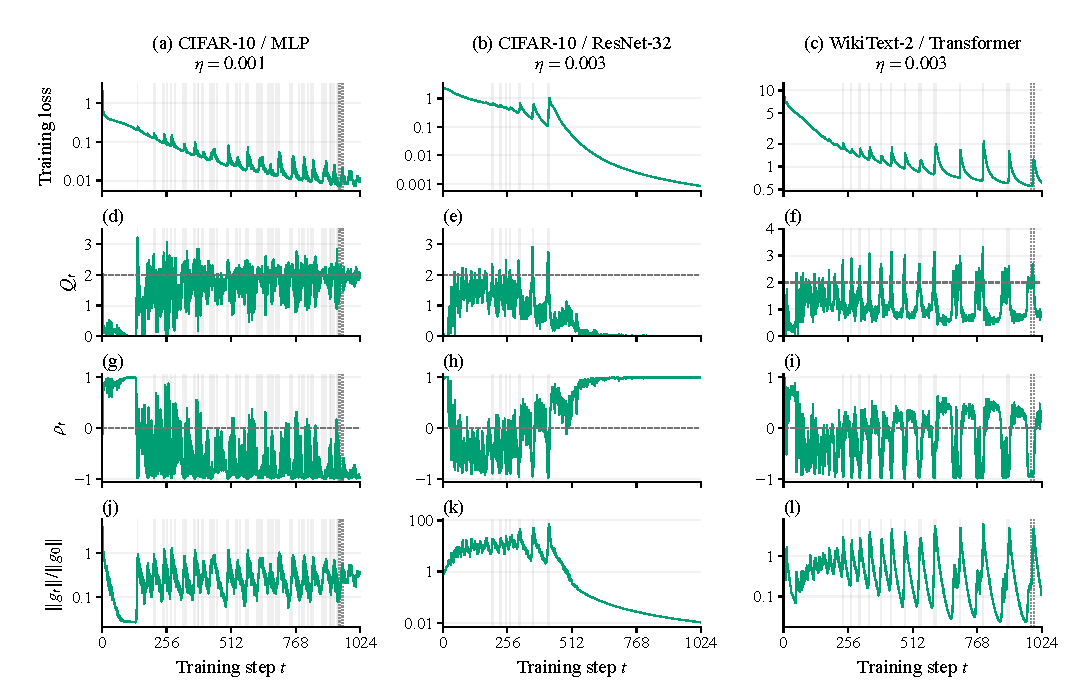
\includegraphics[width=\textwidth]{figures/00-high-lr-overview-cifar10-mlp-resnet-wikitext2-transformer.pdf}
\caption{Loss spikes and consecutive-gradient behavior under full-objective Adam. Columns are MLP, ResNet-32, and Transformer, at learning rates $.001/.003/.003$, with one initialization per model. Rows show loss, the gradient-projected response $\eta\widehat\kappa_t$, consecutive-gradient cosine, and gradient norm relative to initialization. Filled gray bands mark the rising portions of recovered loss excursions exceeding 10\%; outlined bands mark excursions whose recovery is not observed. Events are selected from loss alone. Training step $t$ counts completed updates; gradient measurements are made at $\theta_t$, before the next update. Loss is recorded through 1,024 updates and gradients through 1,023. The $\eta\widehat\kappa_t$ axis starts at zero; negative values lie outside its displayed range.}
\label{fig:adam-overview}
\end{figure*}

Unlike the sustained GD oscillations, the Adam trajectories exhibit
distinct excursions and recoveries. This is consistent with the adaptive
preconditioner mechanism analyzed by Bai et al.~\cite{bai2026spikes}:
changing second moments can alter the effective step size independently
of changes in the underlying Hessian. Our measurements describe how the
resulting motion appears in consecutive gradients. Early constructive
intervals give way to persistent reversal.
Prominent excursions occur with negative cosine and growing gradient
norms, producing large peaks in $\eta\widehat\kappa_t$. In ResNet and
Transformer, recovery often includes renewed constructive alignment and
falling norms.

The loss can reach lower values after an excursion. Such an excursion
could accompany movement into another basin, while momentum can delay
the update's response to a newly changing gradient direction. Whether
that movement helps depends on the current landscape, architecture,
and optimizer state. Related work on SGD catapults shows that spikes can
accompany improved feature learning~\cite{zhu2024catapults}; their role
under Adam must likewise be evaluated together with subsequent progress.

After computing the raw gradient, but before applying the next update,
we may want to classify whether that update will increase the loss.
Let $L_t=\mathcal L(\theta_t)$ and define an increase as
$(L_{t+1}-L_t)/L_t\geq0.001$. At decision step $t$, both $g_t$ and $L_t$
are available. However, the pair $(g_{t-1},g_t)$ describes the response
to the preceding update, from $\theta_{t-1}$ to $\theta_t$. Using it to
classify the outgoing update tests whether that response carries forward.
For quadratic full-batch plain GD, the strict condition
$\eta\widehat\kappa_t>2$ exactly characterizes a positive loss change
on the preceding step. This exact retrospective equivalence does not
extend to a finite nonlinear step or to Adam, whose applied direction
also depends on its moments.

Table~\ref{tab:severity} compares the gradient conditions with the
simple history rule $L_t>L_{t-1}$. Accuracy is the fraction of all
decisions classified correctly. Warning hit rate is the fraction of
warnings followed by an increase; lift divides this rate by the overall
frequency of increases. Together they distinguish correct classification
from how informative an issued warning is.

\begin{table*}[!t]
\centering\small
\caption{Before-update diagnostics for a next-step loss increase of at least 0.1\%. All 1,023 decisions per model are retained. Acc. is classification accuracy, $(\mathrm{TP}+\mathrm{TN})/1023$; Hit is the percentage of warnings followed by the target (precision); lift is Hit divided by the baseline event rate. The no-increase baseline exposes class imbalance. The last two conditions agree on these data and are two forms of the same diagnostic.}
\label{tab:severity}
\setlength{\tabcolsep}{4pt}
\begin{tabular}{@{}lrrrrrrrrr@{}}
\toprule
& \multicolumn{3}{c}{MLP} & \multicolumn{3}{c}{ResNet} & \multicolumn{3}{c}{Transformer} \\
Condition & Acc. (\%) & Hit (\%) & Lift ($\times$) & Acc. (\%) & Hit (\%) & Lift ($\times$) & Acc. (\%) & Hit (\%) & Lift ($\times$) \\
\midrule
Baseline event rate & \multicolumn{3}{c}{446/1023 (43.6\%)} & \multicolumn{3}{c}{88/1023 (8.6\%)} & \multicolumn{3}{c}{142/1023 (13.9\%)} \\
\midrule
Always predict no increase & 56.4 & -- & -- & 91.4 & -- & -- & 86.1 & -- & -- \\
Always predict increase & 43.6 & 43.6 & 1.00 & 8.6 & 8.6 & 1.00 & 13.9 & 13.9 & 1.00 \\
$L_t>L_{t-1}$ & 58.1 & 51.9 & 1.19 & 89.0 & 36.8 & 4.28 & 86.5 & 51.3 & 3.70 \\
$\rho_t<0$ & 54.4 & 48.8 & 1.12 & 77.9 & 27.0 & 3.14 & 61.6 & 25.9 & 1.87 \\
$\|g_t\|>\|g_{t-1}\|$ & 53.5 & 47.3 & 1.08 & 68.7 & 14.2 & 1.65 & 63.1 & 22.1 & 1.59 \\
$\rho_t<-\|g_{t-1}\|/\|g_t\|$ & 59.9 & 55.8 & 1.28 & 92.0 & 58.3 & 6.78 & 87.2 & 53.7 & 3.87 \\
$\eta\widehat\kappa_t\geq2$ & 59.9 & 55.8 & 1.28 & 92.0 & 58.3 & 6.78 & 87.2 & 53.7 & 3.87 \\
\bottomrule
\end{tabular}
\end{table*}


The \emph{destructive loss-spike condition} combines reversal with
sufficient gradient growth, $\rho_t<0$ and
$\|g_t\|/\|g_{t-1}\|>-1/\rho_t$. It gives higher accuracy and warning
lift than the previous-loss-rise rule in all three cases. Reversal or
norm growth alone is less selective. The angle/norm condition is
algebraically equivalent to $\eta\widehat\kappa_t>2$; their identical
table entries verify the two implementations, rather than constitute
independent evidence. The non-strict threshold gives the same flags
here because no observed value equals two. The warning lifts are
$1.28\times$, $6.78\times$, and $3.87\times$ for MLP, ResNet, and
Transformer. These signals contain information before the next update,
although the gains in overall accuracy over always predicting no
increase are modest.

A loss curve and a whole-network gradient still leave an important
question unanswered: what is changing inside the network during these
oscillations? We next examine that functional expression directly.

\subsection{Tracing Oscillations through the Learned Function}
\label{subsec:tracing}

A parameter update changes the representations computed inside the
network and, eventually, its output. We trace these changes backwards
from the output toward the input-side layers, asking where they reverse,
how large they become, and whether different parts of the network share
their timing. We compare the same inputs at successive training states;
otherwise, a representation difference could arise simply because the
examples changed. The reference sets are all 5,000 MLP training images,
one original 1,000-image ResNet normalization group, and 64 Transformer
sequences with 2,240 unchanged token positions (Table~\ref{tab:setup}).

A training state $\theta_t$ is the parameter state after $t$ completed
updates. For a window $a{:}b$, we analyze the $T_w=b-a+1$ representation
changes ending at steps $a,\ldots,b$. Computing their consecutive
cosines requires states $a-2,\ldots,b$: the first cosine compares the
changes ending at $a-1$ and $a$.

A measured \emph{site} is a named output in the computation graph.
It can be a single layer, an attention module, or the end of a residual
block group; we record that output rather than averaging internal layers.
Write its activation matrix as $A_t^\ell\in\mathbb R^{N_\ell\times m_\ell}$.
The $N_\ell$ rows identify reference examples and, where relevant, spatial or token
positions; columns identify the $m_\ell$ features at each position.
The preceding update changes this representation by
\begin{equation}
 \delta_t^\ell=\operatorname{vec}(A_t^\ell-A_{t-1}^\ell)
 \in\mathbb R^{P_\ell},\qquad P_\ell=N_\ell m_\ell.
 \label{eq:representation-change}
\end{equation}
Each flattened coordinate is one feature's response at one matching
input position. No examples or features are averaged before measuring
the change. Its direction and size are measured using
\begin{equation}
 c_t^\ell=
 \frac{\langle\delta_{t-1}^\ell,\delta_t^\ell\rangle}
 {\|\delta_{t-1}^\ell\|\|\delta_t^\ell\|},\qquad
 a_t^\ell=\frac{\|\delta_t^\ell\|}{\sqrt{P_\ell}}.
 \label{eq:representation-motion}
\end{equation}
A negative $c_t^\ell$ means the new functional change opposes the
preceding one; positive values indicate reinforcement. As $\rho_t$ measures alignment between consecutive raw gradients,
$c_t^\ell$ measures alignment between consecutive functional changes at
site $\ell$, giving a representation counterpart of constructive and
destructive regimes. The root-mean-square (RMS) displacement $a_t^\ell$
measures the change per coordinate. A zero change has undefined cosine.

The representation counterpart of normalized displacement is
\begin{equation}
 R_{a:b}^\ell=
 \frac{\|\sum_{t=a}^b\delta_t^\ell\|}{\sum_{t=a}^b\|\delta_t^\ell\|}
 =\frac{\|A_b^\ell-A_{a-1}^\ell\|_F}
 {\sum_{t=a}^b\|A_t^\ell-A_{t-1}^\ell\|_F}.
 \label{eq:representation-retention}
\end{equation}
This ratio lies in $[0,1]$ whenever movement occurs: it compares net
displacement with total distance traveled. In the windows below, output
retention is only 1.71\%/2.44\%/3.51\% for MLP/ResNet/Transformer;
the first measured sites retain 3.25\%/3.72\%/24.33\%, respectively.
Together with negative cosines, these values show substantial
back-and-forth movement with little remaining net displacement,
motivating control of its magnitude. Retention measures displacement,
rather than learning quality; orthogonal changes can also produce a
small ratio. All values use the full changes, without mode truncation.

For each site separately, collect the
changes at steps $a,\ldots,b$ into
$D_\ell\in\mathbb R^{T_w\times P_\ell}$, where $T_w=b-a+1$.
Each row is $(\delta_t^\ell)^\top$, and each column follows one fixed
input-position/feature coordinate across updates. A single singular
value decomposition (SVD) fits the whole window,
\begin{equation}
 D_\ell=U_\ell\Sigma_\ell V_\ell^\top.
 \label{eq:temporal-svd}
\end{equation}
The columns $v_{\ell,j}$ of $V_\ell$ are orthonormal patterns of
representation change. A pattern specifies which coordinates change
together and in what proportions. Its coefficient varies in magnitude
and sign from one update to the next. The diagonal entries
$\sigma_{\ell,j}$ of $\Sigma_\ell$ are nonnegative singular values,
ordered from largest to smallest, and $U_\ell$ describes their temporal
variation. Specifically,
\begin{equation}
 \delta_t^\ell=\sum_j\alpha_{t,j}^\ell v_{\ell,j},\qquad
 \alpha_{t,j}^\ell=\sigma_{\ell,j}U_{\ell,(t-a+1),j}.
 \label{eq:pattern-reconstruction}
\end{equation}
A \emph{mode} is the right singular vector
$v_{\ell,j}\in\mathbb R^{P_\ell}$: the $j$th fixed pattern at site $\ell$
over the whole window. Its coordinates span all reference input positions
and features; its indices identify the site and pattern, not a sample
or training step. Equivalently, it is an eigenvector of
$D_\ell^\top D_\ell$ with eigenvalue $\sigma_{\ell,j}^2$.
The rectangular matrix $D_\ell$ itself need not have eigenvectors.
At most $\min(T_w,P_\ell)$ independent patterns can be observed.

The total squared movement is $\|D_\ell\|_F^2=\sum_j\sigma_{\ell,j}^2$.
The fraction captured by the first $k$ patterns is
\begin{equation}
 E_k^\ell=\frac{\sum_{j=1}^k\sigma_{\ell,j}^2}
 {\sum_j\sigma_{\ell,j}^2}.
 \label{eq:energy}
\end{equation}
Thus $E_k^\ell=0.95$ means that reconstruction using these $k$ patterns
retains 95\% of squared movement, leaving 5\% squared reconstruction
error. This quantity is often called cumulative energy, with
``cumulative'' referring to patterns, not steps. We use squared movement
instead of variance because the change matrix is not centered: a
persistent drift is part of the movement being measured. Row norms are
also retained, so larger changes contribute more.

To compare timing across sites of different widths, we compare the
columns of $U_\ell$, whose coordinates always index the same training
steps. Write $U_{\ell,k}$ for the first $k$ columns of $U_\ell$. With $F$ denoting the final network output, their leading-$k$ overlap is
\begin{equation}
 O_k(\ell,F)=\frac{\|U_{\ell,k}^{\top}U_{F,k}\|_F^2}{k}.
 \label{eq:overlap}
\end{equation}
It measures how much of a site's leading time histories lies in the
subspace spanned by the final output's leading time histories. A value of one means the same temporal subspace,
even if the individual basis vectors differ; zero means orthogonal
temporal subspaces. We use $k=10$ within the numerical ranks. This measures shared timing, without backpropagating outputs or
equating feature directions at different sites.

Algorithm~\ref{alg:trace} assembles these measurements.

\begin{algorithm}[H]
\caption{Tracing representation changes through a network}
\label{alg:trace}
\begin{algorithmic}[1]
\Require Training trajectory; ordered reference examples; measured sites; window $a{:}b$
\State Evaluate the same examples at states $a-2,\ldots,b$, preserving normalization groups and training state.
\For{each measured site $\ell$}
 \State Compute consecutive activation differences $\delta_t^\ell$.
 \State Measure change cosine $c_t^\ell$ and RMS displacement $a_t^\ell$; align them with loss at step $t$.
 \State Stack changes $a{:}b$ as rows of $D_\ell$ and compute $R_{a:b}^\ell$.
 \State Decompose $D_\ell D_\ell^\top$ to obtain movement energies and signed coefficient histories.
\EndFor
\State Compute temporal overlap $O_k(\ell,F)$ with the final network output.
\State Analyze the raw gradients used by the same updates separately.
\end{algorithmic}
\end{algorithm}

\begin{figure*}[!t]
\centering
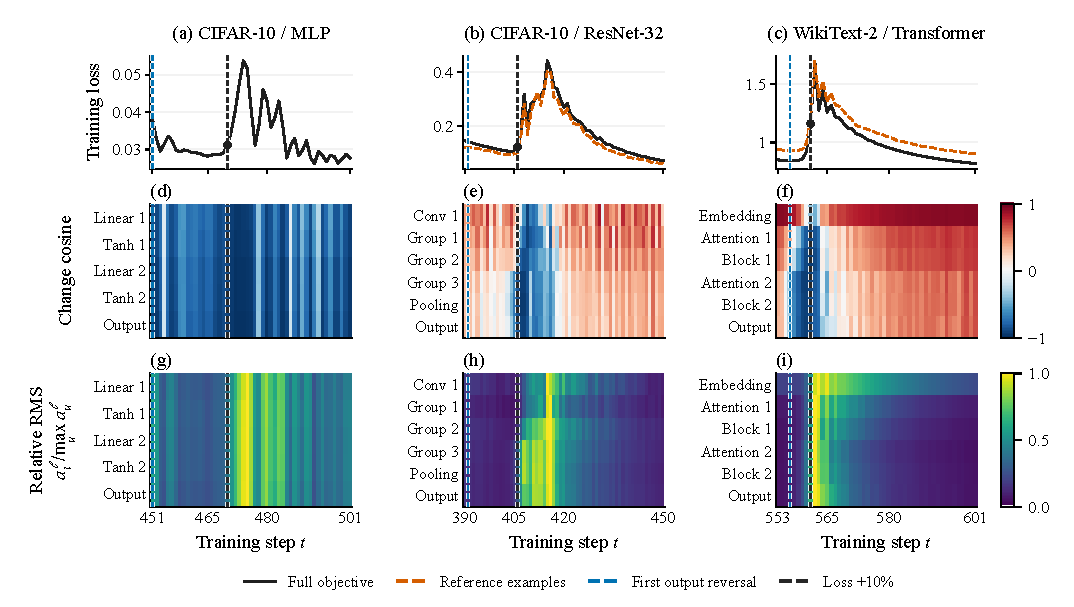
\includegraphics[width=\textwidth]{figures/00-three-model-loss-representation-motion.pdf}
\caption{Loss and representation changes in selected Adam windows: steps 451--501 (MLP), 390--450 (ResNet), and 553--601 (Transformer). Top: complete training loss and loss on the reference examples. Middle: cosine between consecutive representation changes; blue denotes reversal and red denotes reinforcement. Bottom: relative RMS displacement $a_t^\ell/\max_{u\in[a,b]}a_u^\ell$, normalized separately within each site and displayed window. The 5/6/6 rows are measured site outputs, not averages of internal layers. Reference sets contain 5,000 images, one original 1,000-image BatchNorm group, and 2,240 token positions. Blue dashed lines mark the first displayed negative output-change cosine; the MLP is already negative at entry. Black dashed lines mark the first loss at least 10\% above the pre-peak minimum. These lines compare timing; they do not identify a unique initiating event.}
\label{fig:trace-motion}
\end{figure*}

Figure~\ref{fig:trace-motion} shows where functional oscillation appears
and how its size changes. The top row locates the loss excursion.
Reading the cosine maps backwards from output to input reveals how
widely reversal is shared. In the MLP, every displayed change has
negative cosine at every measured site, from the first linear input
map to the final output. Oscillation is therefore homogeneous across
the measured depth, even while loss rises and falls. The RMS maps add
its changing amplitude. Comparing pre- and post-nonlinearity measurements
shows that tanh attenuates displacement; each site's separate
normalization in the figure highlights timing rather than absolute
differences in magnitude across sites.

ResNet and Transformer exhibit a less homogeneous pattern. Their
output-side representations reverse while earlier representations can
continue to reinforce their preceding change. The first displayed output
reversal precedes the 10\% loss marker by 15 steps in ResNet and five
in Transformer. In ResNet, the first convolution reaches its largest
displacement at the loss peak, followed one step later by the remaining
displayed sites. In Transformer, the embedding becomes more oscillatory
near the large excursion and returns to constructive movement sooner
than the later sites. Larger backpropagated errors could recruit earlier
representations into stronger changes, while constructive intervals
could accumulate smaller changes before that reorganization. This
architecture-dependent interpretation motivates examining both the
direction and magnitude throughout the network.

\begin{figure*}[!t]
\centering
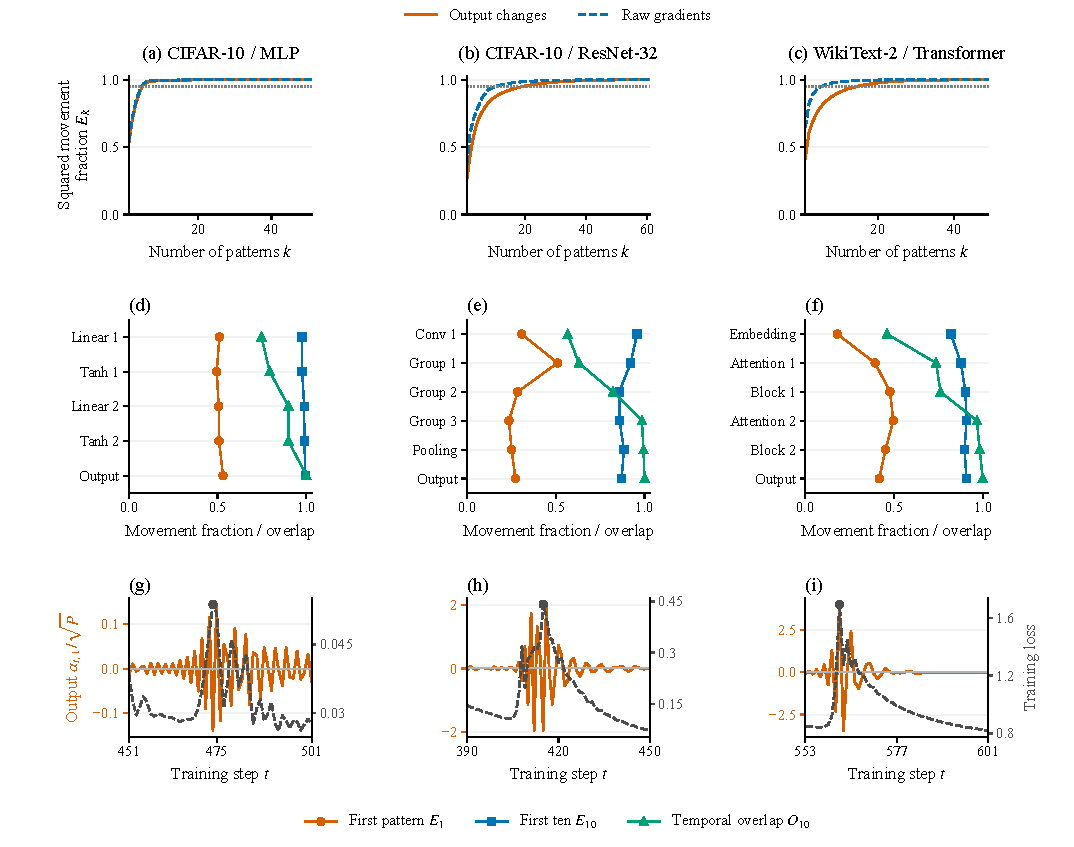
\includegraphics[width=\textwidth]{figures/01-three-model-temporal-structure.pdf}
\caption{Patterns and timing of representation movement in the same windows as Fig.~\ref{fig:trace-motion}, containing 51/61/49 changes. Top: cumulative fraction of squared movement for output changes and for the raw gradients used by those updates; the dotted line marks 95\%. Middle: each site's fraction in its first pattern ($E_1^\ell$) and first ten ($E_{10}^\ell$), and temporal overlap with the output ($O_{10}$). Bottom: signed coefficient of the leading output pattern, divided by $\sqrt P$ to express its coordinate RMS scale. A coefficient crossing zero reverses direction along that fixed pattern. Energy, temporal overlap, and signed motion answer different questions; none alone establishes causal transmission through a layer.}
\label{fig:trace-structure}
\end{figure*}

Figure~\ref{fig:trace-structure} asks whether these changes repeatedly
use a small set of patterns. The top row shows concentration of squared
movement in the leading output modes, alongside the corresponding
gradient decomposition. Concentration can reflect both repeated
directions and a few large changes; the equal-length and orthogonal
controls in Supplementary Section S4 separate these effects.
The middle row extends the analysis through the network: $E_1^\ell$
and $E_{10}^\ell$ show concentration at each site, whereas $O_{10}$ shows
how much its leading temporal structure is shared with the final output.
The selected ResNet window has stronger temporal agreement toward the
output, with shared structure still extending to the input-side sites.
Finally, the bottom row establishes the back-and-forth component that
energy fractions alone cannot establish. Repeated changes in the sign
of $\alpha_{t,1}^F/\sqrt{P_F}$ show reversal along one fixed output
pattern, and its amplitude shows how strongly that pattern moves.

Together, the two figures and the small retention values characterize
coordinated, approximately low-dimensional functional oscillation in
these windows. The temporal Gram matrix $D_\ell D_\ell^\top$ permits
the analysis without storing all spatial modes; implementation and
numerical checks are in Supplementary Section S4. The resulting
intervention question is whether limiting the magnitude of local
representation changes can reduce loss excursions while preserving
subsequent training progress.

% Full-paper adaptation; the separately reviewed V-C fragment remains unchanged.
% Requires amsmath, amssymb, graphicx, booktabs, algorithm, algpseudocode.
\providecommand{\vcassetroot}{../evidence/05-adam/c-intervention}
\subsection{Interventions Guided by Functional Motion}
\label{sec:vc-interventions}

The tracing analysis separates the direction and magnitude of representation
changes. We therefore test whether limiting local displacement can reduce loss
excursions while preserving training progress and allowing reversals. We compare
a local displacement cap with immediate LR reduction, late second-moment
changes, and global gradient clipping.

\begin{figure*}[!t]
\centering
\includegraphics[width=\textwidth]{\vcassetroot/figures/24-main-intervention-tradeoff.pdf}
\caption{Loss variation and training progress for all 33 treated continuations,
each compared with its unchanged Adam control at the origin. Horizontal values
are $100(\bar L/\bar L_{\mathrm{Adam}}-1)$; vertical values are
$100(1-\mathrm{PV}/\mathrm{PV}_{\mathrm{Adam}})$. Leftward and upward changes are
favorable. Axes are model-specific and retain every setting, including increased
variation. This is one initialization per model; settings have unequal effective
strength and are not independent seed replications.}
\label{fig:vc-tradeoff}
\end{figure*}

\input{\vcassetroot/tables/matched-main-outcomes.tex}

\begin{figure*}[!t]
\centering
\includegraphics[width=\textwidth]{\vcassetroot/figures/25-main-q50-functional-motion.pdf}
\caption{Full training loss and fixed-probe motion under unchanged Adam and the
preselected q50 cap. Heatmaps show consecutive-change cosine and displacement
RMS at five MLP and six ResNet/Transformer stage endpoints. Each incoming change
is placed at its completed-step endpoint. Both RMS maps divide by the same
stage-specific maximum under unchanged Adam; the color scale includes every
value. Dashed vertical lines mark the baseline's largest relative loss-excursion
peak within the full window, not treatment triggers. Embed., Attn and Pool denote
embedding, attention output and pooling endpoints. Output motion uses raw MLP
coordinates or cross-entropy log probabilities. No smoothing or stage averaging
is applied.}
\label{fig:vc-motion}
\end{figure*}

\subsubsection{A past-calibrated displacement cap}
For an affine module $Z=HW^\top+\mathbf{1}_n b^\top$, let
$H_s\in\mathbb{R}^{n\times d}$ contain its current fixed-probe inputs,
$W_s\in\mathbb{R}^{m\times d}$ its weights, and $b_s\in\mathbb{R}^m$ its biases.
Rows index examples or token/spatial positions; columns of $Z\in\R^{n\times m}$
index output units. Let $\Delta W_s$ and $\Delta b_s$ be the native stored Adam increments
with the shapes of $W_s$ and $b_s$. Convolution inputs are receptive-field
patches; absent biases have zero increment.
The direct change attributable to this module's update is
\begin{equation}
 \Delta Z_s^{\mathrm{dir}}=H_s\Delta W_s^\top+\mathbf{1}_n \Delta b_s^\top,\qquad
 c_{s,j}=\frac{\|\Delta Z^{\mathrm{dir}}_{s,:,j}\|_2}{\sqrt{n}}.
 \label{eq:vc-score}
\end{equation}
Thus $c_{s,j}$ is one RMS score per output unit across the probe rows,
rather than a worst-case bound for each example. For a positive module budget
$\tau_\ell$, we scale each complete output-unit
weight row and its bias together:
\begin{equation}
 \begin{split}
 a_{s,j}&=\min(1,\tau_\ell/c_{s,j}),\\
 \Delta W^{\mathrm{cap}}_{s,j:}&=a_{s,j}\Delta W_{s,j:},\qquad
 \Delta b^{\mathrm{cap}}_{s,j}=a_{s,j}\Delta b_{s,j}.
 \end{split}
 \label{eq:vc-cap}
\end{equation}
A zero score uses factor one; a zero budget disables that module's cap.
Before treatment at step $f\to f+1$, one scalar budget per module is fixed as
\begin{equation}
 \begin{split}
 \tau_\ell(q)&=\operatorname{Quantile}_q\{c^{\mathrm{native},\ell}_{s,j}\},\\
 &s=f-8,\ldots,f-1,\quad j=1,\ldots,m_\ell.
 \end{split}
 \label{eq:vc-calibration}
\end{equation}
Quantiles use linear interpolation of the pooled scores. The median (q50)
is preselected; q25/q75 test sensitivity. Units whose proposal would induce
larger direct movement are damped proportionally, while smaller proposals
are retained. The budget has activation units and remains fixed as the current
inputs change.

The rule bounds direct affine RMS on the current probe, up to FP32 storage
rounding. Incoming upstream motion and its interaction with the update remain
unconstrained, so total representation motion and loss are not bounded.
Algorithm~\ref{alg:vc-cap} retains native Adam state and untargeted increments.
Scores use a current probe forward to capture $H_s$ and local products with
the proposed increments; each module does not require a second full-network
forward at altered weights. Evaluating propagated motion separately compares
successive probe captures. The controller requires neither temporal SVD nor
a matrix inverse, but its extra forward, products, and bookkeeping have measured
cost. Supplementary Section S5 gives the input-metric interpretation and the
unconstrained upstream terms.

\begin{algorithm}[!b]
\caption{Past-calibrated local displacement cap}
\label{alg:vc-cap}
\begin{algorithmic}[1]
\Require State $\theta_s$, Adam state, fixed probe, targets, fixed budgets $\tau_\ell$
\State Compute the full objective gradient at $\theta_s$.
\State Capture current probe inputs $H_s^\ell$ with the fixed normalization context; preserve random state.
\State Advance native Adam moments/clock and retain the actual stored proposal increments.
\For{each target $\ell$ with $\tau_\ell>0$}
  \State Compute scores by~\eqref{eq:vc-score}; scale weight rows and biases by~\eqref{eq:vc-cap}.
\EndFor
\State Store $\theta_{s+1}$ with untargeted increments unchanged; retain the advanced Adam state.
\State Check direct-score bounds with storage-rounding tolerance; measure propagated motion and loss separately.
\end{algorithmic}
\end{algorithm}

\subsubsection{Matched comparison}
Within each model, all settings share complete model/optimizer/random state,
data order and numerical settings at one initialization. Fixed windows are
$512$--$800$ for CIFAR-10/MLP,
$256$--$576$ for CIFAR-10/ResNet-32, and $544$--$928$ for the two-layer
WikiText-2 Transformer. Training step $s$ counts completed optimizer updates.
Each update uses the complete objective in Table~\ref{tab:setup}, with its
original normalization groups and no dropout.

Unchanged Adam~\cite{kingma2014adam} uses learning rates $.001/.003/.003$,
$\beta_1=.9$, $\beta_2=.999$, $\epsilon=10^{-8}$, and no weight decay.
The four intervention families are immediate LR multipliers $.75/.5/.1$;
late $\beta_2$ values $.95/.9/.5$; global raw-gradient L2 clipping at
$.5/1$~\cite{pascanu2013difficulty}; and distributed q25/q50/q75 caps.
The $\beta_2$ switch retains moments and the step counter, using the new value
in both the recurrence and native $1-\beta_2^{\mathrm{step}}$ correction.
Clipping acts on the complete accumulated raw gradient before Adam.
Caps target both MLP hidden affines, all 31 ResNet convolutions, and the two
QKV and four feed-forward Transformer affines. All 12 conditions per model
start at the same fork; no intervention waits for a later detected spike.

Probes retain the coverage in Table~\ref{tab:setup}.
The full training gradient is unchanged by probe coverage. Every state has loss
and motion measurements. FP32 training/storage and FP64 reductions are matched;
exact native replay checks qualify shared controls across workers.

We report the mean post-fork loss $\bar L$ and positive loss variation,
\begin{equation}
 \bar L=\frac{1}{e-f}\sum_{s=f+1}^{e}L_s,\qquad
 \mathrm{PV}=\sum_{s=f+1}^{e}\max(L_s-L_{s-1},0).
 \label{eq:vc-outcomes}
\end{equation}
PV accumulates upward loss changes, rather than counting excursions.
Final training loss, the last-32-state mean and full held-out losses retain
endpoint context. Held-out evaluations at $f$, $f+32$, midpoint, $e-32$ and $e$
are not used to select checkpoints or settings.

\subsubsection{Excursion suppression and training progress}
Figure~\ref{fig:vc-tradeoff} and Table~\ref{tab:vc-outcomes} separate loss
smoothness from learning progress. Reducing LR to $.1\eta$ removes
$99.6\%$, $99.0\%$, and $100\%$ of PV in MLP/ResNet/Transformer, but increases
ResNet mean loss by $89.5\%$. Late $\beta_2$ changes are model-dependent:
all three worsen MLP mean loss and PV, whereas $\beta_2=.9$ lowers
Transformer mean loss by $16.8\%$. Both clipping thresholds worsen mean loss
and PV in MLP and ResNet. Transformer clipping at $.5$ instead lowers them
by $17.8\%$ and $87.7\%$, respectively.

All nine cap/model combinations lower both mean loss and PV. The lowest observed
mean loss in each model belongs to a cap setting: q50 for MLP/Transformer
and q25 for ResNet. The preselected q50 reduces mean loss by
$32.2\%$, $9.4\%$, and $19.8\%$, with PV reductions of $87.8\%$, $2.8\%$, and $96.2\%$.
Quantile sensitivity is nonmonotone, and the finite-window mean does not establish
better terminal convergence. In particular, ResNet q50 increases final and
last-32 loss by $20.0\%$ and $21.5\%$; q25/q75 improve those endpoints.
The full trajectories and detailed outcomes are retained in the supplementary
comparison.

\subsubsection{Functional effect and limits}
Figure~\ref{fig:vc-motion} shows that q50 lowers the largest output RMS jump
by $83.2\%$, $23.1\%$, and $62.9\%$, while output reversals remain at
$89.2\%$, $66.9\%$, and $95.8\%$ of updates. Their baseline frequencies are
$99.3\%$, $36.9\%$, and $36.7\%$. Smaller extreme jumps therefore coexist with
persistent, sometimes more frequent, reversals. Total squared output motion
falls $88.6\%$ and $55.4\%$ in MLP and Transformer, but rises $39.7\%$
in ResNet. The effect concerns extreme displacements, not uniform suppression
of every measure of motion.

In the previously selected ResNet tracing window, steps $390$--$450$, q50
reduces the maximum loss from $.4407$ to $.1736$ ($60.6\%$).
Later oscillations explain why the complete $256$--$576$ window has only
$2.8\%$ lower PV. This secondary readout connects the intervention to the
traced event while retaining the full horizon as the primary comparison.

\begin{samepage}
For the squared-loss MLP, actual output motion has the exact accounting
\begin{equation}
 L_{s+1}-L_s=\frac{\langle F_s-Y,\Delta F_s\rangle}{N}
             +\frac{\|\Delta F_s\|_F^2}{2N},
 \label{eq:vc-output-loss}
\end{equation}
\end{samepage}
where $\Delta F_s=F_{s+1}-F_s$ and $N=5000$. For all 161 baseline and
70 q50 output-space loss rises above $10^{-8}$, the linear term is negative
and outweighed by the quadratic term. This is an exact output-space identity;
its linear term need not equal the parameter-space directional derivative.
Cross-entropy requires its own readout. The evidence supports displacement
control with persistent reversals, without identifying a unique causal source.

Training improvements also carry held-out tradeoffs: q50 terminal test loss
increases $0.53\%$, $2.42\%$, and $27.52\%$. These evaluations cover all 10,000
CIFAR-10 test images and 245,550 WikiText-2 test tokens; full validation and
five-state trajectories accompany the supplementary results. The implementation
has measurable cost: in the MLP q50 arm, controller time is $41.8$ ms/update,
compared with $4.4$ ms/full-gradient boundary. Instrumentation and host differences
preclude a time-to-loss claim. These single-initialization continuations use
unequal effective intervention strengths; reliability across initializations,
stochastic deployment and generalization benefits require additional evidence.


\section{Conclusion}
\label{sec:conclusion}

Constructive and destructive regimes connect the interaction of successive gradients to curvature, accumulation, and changes in the learned function. Their interpretation depends on the object and timescale being measured. Negative adjacent interaction can coexist with positive total cross-step interaction and lower loss. Under smooth GD, two existing gradients reveal an exact step-averaged directional Hessian scalar, with explicit sampling and finite-step qualifications. Under Adam, the same observable describes a mixed gradient response; exhaustive timing checks show useful structure without establishing a universal next-step alarm.

Fixed-probe tracing makes the functional expression of these regimes visible. Across the three controlled cases, representation motion concentrates in leading modes, shares temporal structure across measured depth, and repeatedly reverses along fitted output patterns. A local affine-displacement cap then tests the usefulness of that interpretation. Every tested cap quantile reduces mean training loss and positive variation relative to its matched unchanged-Adam control, while the preselected median cap retains frequent reversals. Its ResNet endpoint degradation, held-out losses, and implementation cost prevent interpreting this result as universal optimizer superiority or improved generalization.

The practical implication is to distinguish reversal from excessive movement and to evaluate intervention effects jointly with learning progress. The next evidential steps are matched independent initializations, prospective diagnostics with fixed horizons and loss-history baselines, independent probes and quiet-window controls, and representation-aware comparators with matched tuning budgets. Stochastic deployment and larger-scale evaluation remain separate tests. Within the present scope, the framework provides a reproducible route from observable gradient interaction to a bounded, experimentally evaluated functional control.

\bibliographystyle{IEEEtran}
\bibliography{references}
\end{document}
